\documentclass[12pt]{beamer}

\usetheme{Madrid}
\setbeamertemplate{navigation symbols}{}

\usepackage[brazil]{babel}
\usepackage[utf8]{inputenc}
\usepackage[T1]{fontenc}
\usepackage{lmodern}
\usepackage{amsmath, amssymb}
\usepackage{graphicx}
\usepackage{xcolor}
\usepackage{tikz}
\usetikzlibrary{arrows.meta, positioning, shapes.geometric}
\usepackage{svg}
\usepackage{hyperref}
\usepackage{algpseudocode}   % fornece o ambiente algorithmic
\usepackage{algorithmicx}    % base do algpseudocode

\graphicspath{ {./figuras/} }

% Sumário automático a cada seção
\AtBeginSection[]{
  \begin{frame}{Sumário}
    \tableofcontents[currentsection]
  \end{frame}
}

% ── Metadados ───────────────────────────────────────────────
\title{Animação Física Simplificada em Web}
\subtitle{Trabalho de Conclusão de Curso}
\author[Diego V. S. de Matos]{Diego Vasconcelos Schardosim de Matos}
\institute[UFRJ]{Universidade Federal do Rio de Janeiro\\Instituto de Computação}
\date{\today}
\logo{\includegraphics[height=1cm]{ufrj-vertical-cor-rgb-telas.png}}

% ============================================================
\begin{document}
% ============================================================

\maketitle

% ============================================================
\section{Introdução}
% ============================================================

\begin{frame}{Motivação}
  \begin{columns}
    \column{0.49\textwidth}
      \begin{itemize}
        \item Jogos
        \item Simulações
        \item Robótica
        \item Desafio educacional e técnico
      \end{itemize}
    \column{0.49\textwidth}
      \begin{figure}
        \centering
        \includegraphics[width=\textwidth]{Unreal-Engine-4.23-Chaos.jpg}
      \end{figure}
  \end{columns}
\end{frame}

% ── Pipeline ────────────────────────────────────────────────
\begin{frame}{Pipeline de Animação Física}
  \begin{center}
    \scalebox{0.8}{
      \begin{tikzpicture}[
          node distance=0.4cm and 0.5cm,
          box/.style={rectangle, draw, rounded corners=4pt,
                      fill=structure!20, minimum width=2.2cm,
                      minimum height=1.0cm, font=\small, align=center},
          arr/.style={-{Stealth[length=7pt]}, thick}
        ]
        \node[box] (A) {Corpos};
        \node[box, right=of A] (B) {Integração\\numérica};
        \node[box, right=of B] (C) {Detecção\\de colisão};
        \node[box, right=of C] (D) {Resposta\\a colisão};
        \node[box, right=of D] (E) {Renderização\\(Opcional)};

        \draw[arr] (A) -- (B);
        \draw[arr] (B) -- (C);
        \draw[arr] (C) -- (D);
        \draw[arr] (D) -- (E);
        \draw[arr] (E.south) -- ++(0,-0.5) -| (A.south);
      \end{tikzpicture}
    }
  \end{center}
  \vspace{0.4cm}
  \begin{alertblock}{}
      \footnotesize
      Motores de referência: Havok, PhysX, Bullet, Box2D. Todos inspiram a proposta Web deste trabalho.
  \end{alertblock}
  % \begin{center}
  %   Baseado no método de \textbf{Jakobsen}~\cite{jakobsen2001advanced}, restrições geométricas, sem torques nem tensores de inércia.
  % \end{center}
\end{frame}

% ============================================================
\section{Animação Baseada em Física}
% ============================================================

% ── Keyframe vs física ──────────────────────────────────────
\begin{frame}{\textit{Keyframe} vs.\ Baseada em Física}
  \begin{columns}[c]
    \column{0.49\textwidth}
      \begin{figure}
        \centering
        \includegraphics[width=\linewidth]{blender-3d-keyframe-animation.jpg}
      \end{figure}
    \column{0.49\textwidth}
      \begin{figure}
        \centering
        \includegraphics[width=\linewidth]{thumbnail-Sculpt-Sim-Pose-BN.jpg}
      \end{figure}
  \end{columns}
  \vspace{0.3cm}
  \begin{alertblock}{}
    \centering Objetivo: \textbf{plausibilidade visual}, não precisão científica.
  \end{alertblock}
\end{frame}

% ── Partículas ───────────────────────────────────────────────
\begin{frame}{Partículas}
  \begin{columns}[c]
    \column{0.45\textwidth}
      Não simulamos o objeto como um todo, simulamos cada \textbf{partícula} que o compõe.
      \vspace{0.4cm}
      \begin{itemize}
        \item Posição $\vec{x}$
        \item Forças aplicadas (ex: gravidade $\vec{g}$)
      \end{itemize}
    \column{0.52\textwidth}
      \begin{figure}
        \centering
        \includesvg[width=0.7\textwidth]{particulas}
      \end{figure}
  \end{columns}
\end{frame}
 
% ── Formas Geométricas ───────────────────────────────────────
\begin{frame}{Formas Geométricas}
  \begin{columns}[c]
    \column{0.45\textwidth}
      Um objeto é um conjunto de \textbf{partículas} associado a
      uma \textbf{forma geométrica}.
 
      \vspace{0.4cm}
      Neste trabalho: apenas \textbf{formas convexas}.
    \column{0.52\textwidth}
      \begin{figure}
        \centering
        \includesvg[width=0.7\textwidth]{grupo-particulas}
      \end{figure}
  \end{columns}
\end{frame}

% ── Restrições ───────────────────────────────────────────────
\begin{frame}{Restrições Geométricas}
  \begin{columns}[c]
    \column{0.40\textwidth}
      \[
        |\vec{x}_i - \vec{x}_j| = d
      \]
      \vspace{0.4cm}
      Após cada passo, partículas são \textbf{projetadas} de volta.
    \column{0.57\textwidth}
      \begin{figure}
        \centering
        \includesvg[width=\textwidth]{restricao-linear}
      \end{figure}
  \end{columns}
\end{frame}

% ── Relaxamento ─────────────────────────────────────────────
\begin{frame}{Resolvendo Restrições por Relaxamento}
  \begin{columns}
    \column{0.5\textwidth}
      Resolver localmente e repetir $\approx$ \textbf{3 a 5 vezes} converge o sistema global.
  
    \column{0.5\textwidth}
      \begin{algorithmic}[1]
        \State $\vec{\delta} \leftarrow \vec{x}_2 - \vec{x}_1$
        \State $c \leftarrow \dfrac{\|\vec{\delta}\| - d}{\|\vec{\delta}\|}$
        \State $\vec{x}_1 \leftarrow \vec{x}_1 - \epsilon\,\vec{\delta}\,c$
        \State $\vec{x}_2 \leftarrow \vec{x}_2 + \epsilon\,\vec{\delta}\,c$
      \end{algorithmic}
  \end{columns}
\end{frame}

% ── Corpos ──────────────────────────────────────────────────
\begin{frame}{Representação dos Corpos}
  \begin{figure}
    \includegraphics[width=0.9\textwidth]{physics-of-jellycar.png}
  \end{figure}
\end{frame}

% ── Estrutura topológica ─────────────────────────────────────
\begin{frame}{Estrutura Topológica do Tecido}
  \begin{columns}[c]
    \column{0.38\textwidth}
      \begin{enumerate}
        \item \textbf{Estruturais}\\horizontal/vertical
        \item \textbf{Cisalhamento}\\diagonal
        \item \textbf{Flexão}\\vizinho alternado
      \end{enumerate}
    \column{0.60\textwidth}
      \begin{tikzpicture}[scale=0.92]
        \foreach \x in {0,1,2,3} \foreach \y in {0,1,2,3}
          \filldraw[black] (\x,\y) circle (2.5pt);
        % Estruturais
        \foreach \x in {0,1,2} \foreach \y in {0,1,2,3}
          \draw[black, thick] (\x,\y) -- (\x+1,\y);
        \foreach \x in {0,1,2,3} \foreach \y in {0,1,2}
          \draw[black, thick] (\x,\y) -- (\x,\y+1);
        % Cisalhamento
        \foreach \x in {0,1,2} \foreach \y in {0,1,2} {
          \draw[gray, dashed, thin] (\x,\y) -- (\x+1,\y+1);
          \draw[gray, dashed, thin] (\x+1,\y) -- (\x,\y+1);
        }
        % Flexão
        % \foreach \x in {0,1} \foreach \y in {0,1,2,3}
        %   \draw[blue!60, thick, dotted] (\x,\y) -- (\x+2,\y);
        % \foreach \x in {0,1,2,3} \foreach \y in {0,1}
        %   \draw[blue!60, thick, dotted] (\x,\y) -- (\x,\y+2);
        % Legenda
        \draw[black, thick]           (4.4,2.8) -- (5.0,2.8) node[right, font=\tiny]{Estrutural};
        \draw[gray, dashed, thin]     (4.4,2.3) -- (5.0,2.3) node[right, font=\tiny]{Cisalham.};
        % \draw[blue!60, thick, dotted] (4.4,1.8) -- (5.0,1.8) node[right, font=\tiny]{Flexão};
      \end{tikzpicture}
  \end{columns}
\end{frame}

% ============================================================
\section{Detecção de Colisões}
% ============================================================

% ── SAT ─────────────────────────────────────────────────────
\begin{frame}{Teorema do Eixo Separador (SAT)}
  \begin{columns}[c]
    \column{0.42\textwidth}
      As projeções de $A$ e $B$ estão sempre em lados opostos de um plano separador.
    \column{0.55\textwidth}
      \begin{figure}
        \centering
        \includesvg[width=0.80\linewidth]{eixo-separador}
        % Figura existente: aresta em amarelo, eixo separador
        % perpendicular, intervalos de projeção separados
      \end{figure}
  \end{columns}
\end{frame}

% ── Minkowski ───────────────────────────────────────────────
\begin{frame}{Algoritmo de Gilbert-Johnson-Keerthi (GJK)}
  \begin{figure}
    \centering
    \includesvg[width=0.9\linewidth]{soma-minkowski}
  \end{figure}

  \[
    A - B = A + (-B) = \{\,\vec{x}{-}\vec{y} \mid \vec{x}{\in}A,\,\vec{y}{\in}B\,\}
  \]
  \vspace{0.3cm}
  \[
    A \cap B \neq \emptyset \;\iff\; \mathbf{0} \in A{-}B
  \]
\end{frame}

\begin{frame}{Função Suporte}
  \begin{columns}
    \column{0.4\textwidth}
      \[
        S_A(\vec d) = \arg\max_{\vec a \in A} (\vec d \cdot \vec a)
      \]
      \[
        S_{A-B}(\vec{d}) = S_A(\vec{d}) - S_B(-\vec{d})
      \]
    \column{0.55\textwidth}
      \begin{figure}
        \centering
        \includesvg[width=\linewidth]{support-function}
      \end{figure}
  \end{columns}
\end{frame}

% ── Simplex ──────────────────────────────────────────────────
\begin{frame}{GJK — Construção Iterativa do Simplex}
  \begin{columns}[c]
    \column{0.35\textwidth}
      A cada passo adiciona $\vec{s} = S_{A-B}(\vec{d})$:
      \vspace{0.3cm}
      \begin{itemize}
        \item $\vec{s}\cdot\vec{d} \leq 0$\\
              $\Rightarrow$ \textbf{sem colisão}
        \item Origem dentro do simplex\\
              $\Rightarrow$ \textbf{colisão}
      \end{itemize}
    \column{0.62\textwidth}
      \begin{figure}
        \centering
        \includesvg[width=\linewidth]{simplex}
        % Figura existente: 0-simplex, 1-simplex, 2-simplex
      \end{figure}
  \end{columns}
\end{frame}

% ── Ericson 1-simplex ────────────────────────────────────────
\begin{frame}{Subalgoritmo de Ericson — 1-simplex}
  % NOTA: Ericson usa "regiões de Voronoi" de forma equivocada;
  % o correto é apenas "regiões".
  \begin{columns}[c]
    \column{0.32\textwidth}
      Três regiões do segmento $RS$:
      \vspace{0.3cm}
      \begin{itemize}
        \item Região de $R$
        \item Região de $S$
        \item Região da aresta
      \end{itemize}
      \vspace{0.3cm}
      {\small Regiões de vértice\\$\Rightarrow$ \textbf{sem colisão}.}
    \column{0.65\textwidth}
      \begin{figure}
        \centering
        \includesvg[width=\linewidth]{gjk-ericson-1simplex.svg}
        % Figura existente: segmento RS com as três regiões e origem
        % indicada em diferentes posições possíveis
      \end{figure}
  \end{columns}
\end{frame}

% ── Ericson 2-simplex ────────────────────────────────────────
\begin{frame}{Subalgoritmo de Ericson — 2-simplex}
  \begin{columns}[c]
    \column{0.32\textwidth}
      7 regiões $\to$ verificar \textbf{3}:
      \vspace{0.3cm}
      \begin{itemize}
        \item Aresta $\vec{rs}$
        \item Aresta $\vec{rt}$
        \item Interior $\triangle RST$\\
              $\Rightarrow$ \textbf{colisão}
      \end{itemize}
    \column{0.65\textwidth}
      \begin{figure}
        \centering
        \includesvg[width=\linewidth]{gjk-ericson-2simplex.svg}
        % Figura existente: triângulo RST com regiões delimitadas
        % e setas de verificação de aresta rs e rt
      \end{figure}
  \end{columns}
\end{frame}

% ============================================================
\section{Resposta a Colisões}
% ============================================================

% ── Manifold ────────────────────────────────────────────────
\begin{frame}{Conceitos}
  \begin{columns}[c]
    \column{0.5\textwidth}
      \textbf{Pontos de Contato}
      
      Inferidos a partir da região de intersecção entre dois objetos.

    \column{0.5\textwidth}
      \textbf{Manifold de Colisão}
      
      \begin{itemize}
        \item Normal $\hat{n}$
        \item Profundidade $d$
        \item Pontos de contato
      \end{itemize}
  \end{columns}
\end{frame}

% ── SAT MTV ─────────────────────────────────────────────────
\begin{frame}{SAT com MTV}
  \begin{columns}[c]
    \column{0.40\textwidth}
      Testar \textbf{todos} os eixos.\\
      Guardar o de \textbf{menor sobreposição}
      $\Rightarrow$ $\hat{n}$ e $\delta$.
    \column{0.57\textwidth}
      \begin{figure}
        \centering
        \includegraphics[width=0.8\textwidth]{eixo-separador-2.png}
      \end{figure}
  \end{columns}
\end{frame}

% ── EPA ─────────────────────────────────────────────────────
\begin{frame}{EPA — Expansão de Politopos}
  \begin{columns}[c]
    \column{0.40\textwidth}
      GJK detecta colisão mas \textbf{não} fornece $\hat{n}$/$\delta$.\\[0.5cm]
      EPA parte do simplex final do GJK e \textbf{expande} até:
      \[
        \|\vec{w}\| - \|\vec{p}\| < \epsilon
      \]
    \column{0.6\textwidth}
      \begin{figure}
        \centering
        \includegraphics[width=0.9\linewidth, keepaspectratio]{epa.jpg}
        % Figura existente: sequência de iterações do EPA
      \end{figure}
  \end{columns}
\end{frame}

% ── Pontos de contato ────────────────────────────────────────
\begin{frame}{Cálculo dos Pontos de Contato}
  \begin{columns}[c]
    \column{0.49\textwidth}
      \begin{figure}
        \centering
        \includesvg[width=\linewidth]{collision-manifold-2}
        % Figura existente: arestas candidatas em destaque
      \end{figure}
      \begin{center}\small Arestas candidatas\end{center}
    \column{0.49\textwidth}
      \begin{figure}
        \centering
        \includesvg[width=\linewidth]{collision-manifold-3}
        % Figura existente: referência (vermelha) e incidente (azul)
      \end{figure}
      \begin{center}\small Referência (vermelho) e incidente (azul)\end{center}
  \end{columns}
\end{frame}

% ── Separação ───────────────────────────────────────────────
\begin{frame}{Processo de Separação — Vértice-Aresta}
  \begin{columns}[c]
    \column{0.44\textwidth}
      \[
        \vec{c} = d\,\hat{n}, \quad
        \alpha = \frac{(p{-}r)\cdot(s{-}r)}{\|s{-}r\|^2}
      \]
      \[
        p' = p + \vec{c}_A
      \]
      \[
        r' = r + (1{-}\alpha)\,\vec{c}_B, \quad
        s' = s + \alpha\,\vec{c}_B
      \]
    \column{0.53\textwidth}
      \begin{figure}
        \centering
        \includesvg[width=0.85\linewidth]{processo-separacao}
        % Figura existente: p e aresta rs antes/depois da correção,
        % deslocamentos c_A e c_B ponderados por alpha
      \end{figure}
  \end{columns}
\end{frame}

% ── Verlet ──────────────────────────────────────────────────
\begin{frame}{Integração de Verlet}
  \begin{columns}[c]
    \column{0.50\textwidth}
      \[
        \vec{x}_{t+\Delta t} = 2\,\vec{x}_t - \vec{x}_{t-\Delta t}
          + \vec{a}_t\,\Delta t^2
      \]
      \[
        \vec{v}_t \approx \frac{\vec{x}_{t+\Delta t} - \vec{x}_{t-\Delta t}}{2\,\Delta t}
      \]
    \column{0.47\textwidth}
      \begin{exampleblock}{Vantagens}
        \begin{itemize}
          \item Estável sob restrições
          \item Velocidade implícita
        \end{itemize}
      \end{exampleblock}
  \end{columns}
\end{frame}

% ============================================================
\section{Otimizações}
% ============================================================

\begin{frame}{Objetos Delimitadores}
  Simplificar a geometria para testes rápidos de colisão.\\
  
  \begin{figure}
    \centering
    \includesvg[width=\linewidth]{bounding_volumes}
    % Figura existente: esfera, AABB, OBB, K-DOP, fecho convexo
  \end{figure}
\end{frame}

% ── AABB ────────────────────────────────────────────────────
\begin{frame}{AABB — Caixa Delimitadora Alinhada aos Eixos}
  \begin{columns}[c]
    \column{0.52\textwidth}
      \begin{itemize}
        \item Teste de interseção de baixo custo
        \item Ajuste preciso
        \item Cálculo econômico
        \item Fácil de girar e transformar
        \item Baixo consumo de memória
      \end{itemize}
    \column{0.45\textwidth}
      \begin{figure}
        \centering
        \includesvg[width=\linewidth]{fecho-convexo-interseccao}
      \end{figure}
    \end{columns}
\end{frame}

% ── Broad / Narrow ──────────────────────────────────────────
\begin{frame}{Filtragem e Refinamento}
  \begin{columns}[c]
    \column{0.49\textwidth}
      \begin{block}{\centering Fase de Filtragem\\ (Broad Phase)}
        \centering Descartar pares impossíveis usando objetos delimitadores.
      \end{block}
    \column{0.49\textwidth}
      \begin{block}{\centering Fase de Refinamento\\ (Narrow Phase)}
        \centering Usar algoritmos sofisticados como SAT / GJK+EPA apenas nos pares candidatos
      \end{block}
  \end{columns}
\end{frame}

% ── Grade uniforme ───────────────────────────────────────────
\begin{frame}{Filtragem com Grade Uniforme}
  \begin{columns}[c]
    \column{0.44\textwidth}
      \[
        i = \!\left\lfloor \tfrac{x}{C} \right\rfloor\!, \quad
        j = \!\left\lfloor \tfrac{y}{C} \right\rfloor
      \]
      \[
        Key = i + j \times n_{\text{col}}
      \]
      \vspace{0.3cm}
      Candidatos $\Leftrightarrow$ mesma célula.
    \column{0.53\textwidth}
      \begin{figure}
        \centering
        \includesvg[width=0.80\linewidth]{uniform-grid}
        % Figura existente: grade com objetos alocados nas células
      \end{figure}
  \end{columns}
\end{frame}

% ============================================================
\section{Resultados}
% ============================================================

\begin{frame}{Ambiente de Visualização}
  \begin{columns}[c]
    \column{0.49\textwidth}
      \begin{figure}
        \centering
        \includegraphics[width=\textwidth]{demo1.png}
      \end{figure}
    \column{0.49\textwidth}
      \begin{figure}
        \centering
        \includegraphics[width=\textwidth]{demo2.png}
      \end{figure}
  \end{columns}
  
  \begin{center}
    biblioteca typescript $\cdot$ modos SAT e GJK/EPA $\cdot$ p5.js
  \end{center}
  
\end{frame}

% ── Metodologia ─────────────────────────────────────────────
\begin{frame}{Cenários de Teste}
  \begin{columns}[c]
    \column{0.45\textwidth}
      \begin{itemize}
        \item 100 a 1000 objetos (passo 100)
        \item 180 quadros por config.
        \item Sem renderização
        \item \textit{Poisson Disk Sampling}
        \item Ryzen 5 5500U, 24GB RAM DDR4, Ubuntu 24.04LTS
      \end{itemize}
    \column{0.52\textwidth}
      \includegraphics[width=\textwidth]{demo1.png}
    \end{columns}
\end{frame}

% ── Número de testes ─────────────────────────────────────────
\begin{frame}{Impacto da Filtragem}
  \begin{figure}
    \centering
    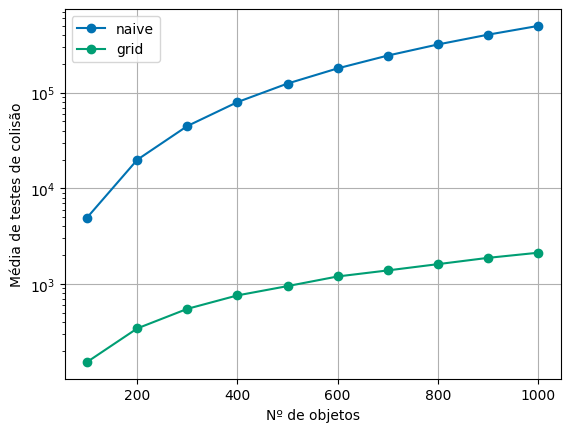
\includegraphics[width=0.9\textwidth]{comparativo-testes-colisao.png}
    % Figura existente: nº de testes de colisão em escala log
  \end{figure}
\end{frame}

% ── Profiling SAT ────────────────────────────────────────────
\begin{frame}{Tempo por Etapa — SAT}
  \begin{figure}
    \centering
    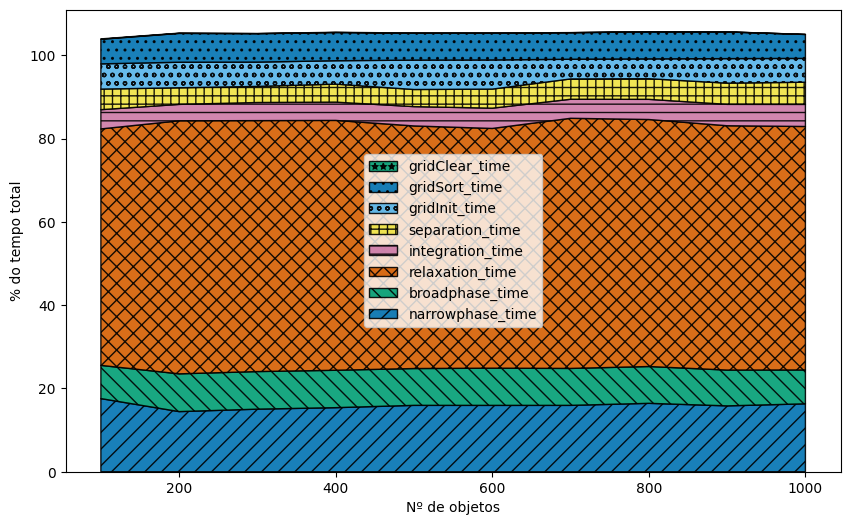
\includegraphics[width=0.9\textwidth]{profiling-sat.png}
    % Figura existente: área empilhada — relaxamento domina
  \end{figure}
\end{frame}

% ── Profiling GJK ────────────────────────────────────────────
\begin{frame}{Tempo por Etapa — GJK/EPA}
  \begin{figure}
    \centering
    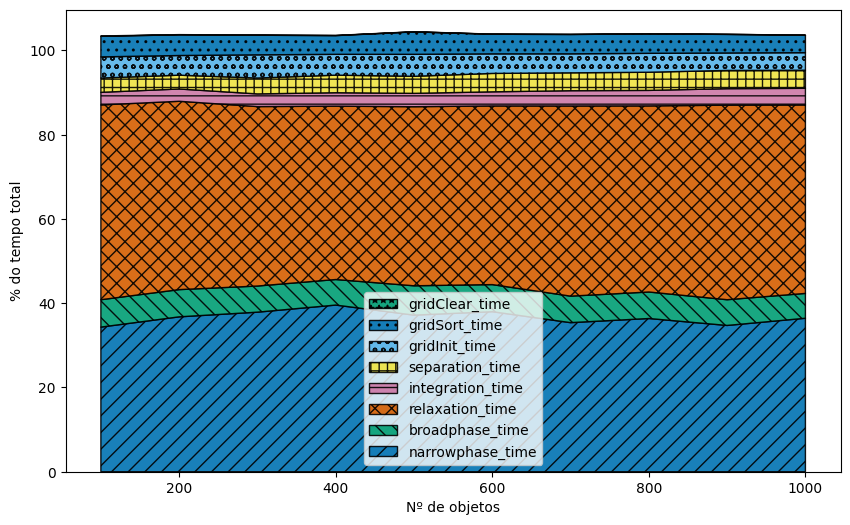
\includegraphics[width=0.9\textwidth]{profiling-gjk.png}
    % Figura existente: área empilhada — GJK com refinamento mais caro
  \end{figure}
\end{frame}

% ── Planck.js ────────────────────────────────────────────────
\begin{frame}{Comparação com \textit{Planck.js}}
  \begin{figure}
    \centering
    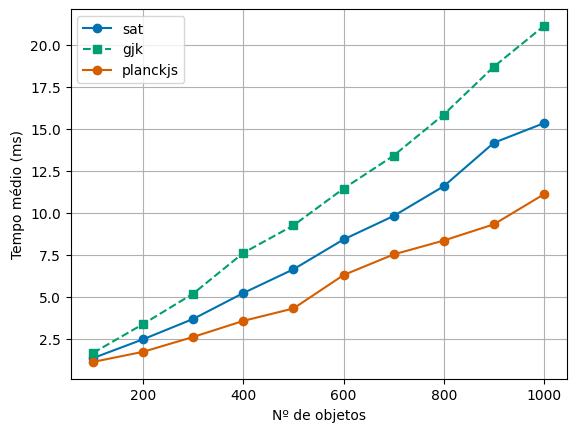
\includegraphics[width=0.9\textwidth]{comparativo-tempo-execução.png}
  \end{figure}
\end{frame}

% ============================================================
\section{Conclusão}
% ============================================================

\begin{frame}{Conclusões e Trabalhos Futuros}
  \begin{columns}[T]
    \column{0.49\textwidth}
      \textbf{Alcançado}
      \begin{itemize}
        \item Motor funcional em TypeScript
        \item SAT, GJK+EPA implementados
        \item Separação geométrica
        \item Filtragem com Grade uniforme
        \item Código aberto e reproduzível
      \end{itemize}
    \column{0.49\textwidth}
      \textbf{Trabalhos Futuros}
      \begin{itemize}
        \item Extensão para 3D
        \item Paralelização com Webworks e WebGPU
        \item BVH / Quadtree na filtragem
      \end{itemize}
  \end{columns}
\end{frame}

% ── Referências ─────────────────────────────────────────────
\begin{frame}{Referências}
  \footnotesize
  \begin{thebibliography}{9}
    \bibitem{jakobsen2001advanced}
      T.~Jakobsen.
      Advanced character physics.
      \textit{GDC}, 2001.
    \bibitem{ericson2004real}
      C.~Ericson.
      \textit{Real-Time Collision Detection}.
      Morgan Kaufmann, 2004.
    \bibitem{bergen2001proximity}
      G.~van den Bergen.
      Proximity queries and penetration depth computation on 3D game objects.
      \textit{GDC}, 2001.
    \bibitem{muratori2016implementingGJK}
      C.~Muratori.
      Implementing GJK.
      \url{https://caseymuratori.com/blog_0003}, 2006.
    \bibitem{collision_manifolds_2017}
      Dyn4j.
      Contact points using clipping.
      \url{https://dyn4j.org/2011/11/contact-points-using-clipping/}, 2011.
  \end{thebibliography}
\end{frame}

% ── Slide final ─────────────────────────────────────────────
\begin{frame}[plain]
  \vfill
  \begin{center}
    {\Large\textbf{Obrigado!}}\\[0.8cm]
    Dúvidas?\\[0.4cm]
    \begin{figure}
      \includesvg[width=4cm]{repo-qrcode}
    \end{figure}
    % \small\url{https://github.com/devdiegomatos/simplified-physics-animation-web}
  \end{center}
  \vfill
\end{frame}

\end{document}